\begin{problem}[Munkres \S58, Ex.\,7(c)]
Let $A$ be a subspace of $X$; let $j\colon A\hookrightarrow X$ be the
inclusion map, and let $f\colon X\to A$ be a continuous map. Suppose there
is a homotopy $H\colon X\times I\to X$ between the map $j\circ f$ and the
identity map of $X$.
\begin{itemize}
\item[(c)] Give an example in which $j_*$ is not an isomorphism.
\end{itemize}
\end{problem}
\begin{proof}[Example]
\renewcommand\qedsymbol{$\spadesuit$}
Consider the following: Write $x_0\coloneqq(1,0)$ and let $f\colon\RR^2\to
S^1$ be the constant map $f(x)\coloneqq e_{x_0}$. This map is continuous by
18.2(a) and and the composition $j\circ f$ is homotopic to $\id_{\RR^2}$
via the homotopy $H(x,t)\coloneqq (1-t)x+t(1,0)$. However, the induced
mapping $j_*\colon\pi_1(S^1,x_0)\to\pi_1(\RR^2,x_0)$ is not an isomorphism
since $\pi_1(S^1,x_0)\cong\ZZ$ while $\pi_1(\RR^2,x_0)=0$.
\end{proof}
\newpage
\begin{problem}[Munkres \S58, Ex.9(a,b,c)]
We define the \emph{degree} of a continuous map $h\colon S^1\to S^1$ as
follows:
\\\\
Let $b_0$ be the point $(0,1)$ of $S^1$; choose a generator $\gamma$ for
the infinite cyclic group $\pi_1(S^1,b_0)$. If $x_0$ is any point of $S^1$,
choose a path $\alpha$ in $S^1$ from $b_0$ to $x_0$ and define
$\gamma(x_0)\coloneqq\hat\alpha(\gamma)$. Then $\gamma(x_0)$ generates
$\pi_1(S^1,x_0)$. The element $\gamma(x_0)$ is independent of the choice of
the path $\alpha$, since the fundamental group of $S^1$ is Abelian.

Now given $h\colon S^1\to S^1$, choose $x_0\in S^1$ and let
$h(x_0)=x_1$. Consider the homomorphism
\[
h_*\colon\pi_1(S^1,x_0)\longrightarrow\pi_1(S^1,x_1).
\]
Since both groups are infinite cyclic, we have
\begin{equation}
\label{eq:1}
\tag{*}
h_*(\gamma(x_0))=d\cdot\gamma(x_1)
\end{equation}
for some integer $d$, if the group is written additively. The integer $d$
is called the \emph{degree} of $h$ and is denoted by $\deg h$.

The degree of $h$ is independent of the choice of the generator $\gamma$;
choosing the other generator woul merely change the sign of both sides of
(\ref{eq:1}).
\begin{enumerate}[label=(\alph*)]
\item Show that $d$ is independent of the choice of $x_0$.
\item Show that if $h,k\colon S^1\to S^1$ are homotopic, they have the same
  degree.
\item Show that $\deg(h\circ k)=(\deg h)\cdot(\deg k)$.
\end{enumerate}
\end{problem}
\begin{proof}
(a) Keeping the same notation as above, let $h\colon S^1\to S^1$ be a
continuous map, $y_0$ be a point in $S^1$ and set $y_1\coloneqq
h(y_0)$. Since $S^1$ is path-connected, there exists a path $\beta\colon
I\to S^1$ from $x_0$ to $y_0$ so that $\alpha*\beta$ is a path from $b_0$
to $y_0$ and
\[
\gamma(y_0)\coloneqq\hat\beta(\gamma(x_0))=\hat\beta\circ\hat\alpha(\gamma)=\widehat{\alpha*\beta}(\gamma)
\]
is a generator for $\pi_1(X,y_0)$. Moreover, the map $h\circ\beta\colon
I\to S^1$ is a path from $x_1$ to $y_1$ and
$\gamma(y_1)\coloneqq\widehat{h\circ\beta}(\gamma(x_1))$ is a generator for
$\pi_1(S^1,y_1)$ so the diagram below commutes
\begin{center}
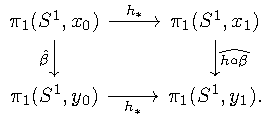
\includegraphics{figures/hw-12-degree-indep}
\end{center}
We check this more explicitly. Let $[f]\in\pi_1(X,x_0)$ then
$\hat\beta([f])=[\bar\beta]*[f]*[\beta]\in\pi_1(X,y_0)$ and
$h_*(\hat\beta([f]))\in\pi_1(S^1,y_1)$. But the latter is just the same as
the loop
\begin{align*}
[h(\bar\beta*f*\beta)]
&=\left[(h\circ\bar\beta)*(h\circ f)*(h\circ\beta)\right]\\
\shortintertext{the above just follows from the definition of the path
  product and is claimed as a fact at the bottom of Munkres, p.\,333}
&=\widehat{h\circ\beta}([hf])\\
&=\widehat{h\circ\beta}\circ h_*([f]).
\end{align*}
Thus, we have that
\begin{equation}
\label{eq:1}
\widehat{h\circ\beta}\circ h_*=h_*\circ\hat\beta.
\end{equation}
Now we move on to the main part of the proof. Let $d$ denote the degree of
the map $h$ when $h_*$ is viewed as a map from $\pi_1(X,x_0)$ to
$\pi_1(X,x_1)$. Then by (\ref{eq:1}) we have
\begin{align*}
h_*(\gamma(y_0))&=
h_*\circ\hat\beta(\gamma(x_0))\\
&=\widehat{h\circ\beta}\circ h_*(\gamma(x_0))\\
&=\widehat{h\circ\beta}(d\gamma(x_1))
\shortintertext{since $\widehat{h\circ\beta}$ is an homomorphism, by
  Theorem 52.1, the latter is equal to}
&=d\left(\widehat{h\circ\beta}(\gamma(x_1))\right)\\
&=d\gamma(y_1).
\end{align*}
Thus, the degree of a continuous map $h\colon S^1\to S^1$ is independent of
the choice of base point.
\\\\
(b) Suppose that $h$ and $k$ are homotopic maps from $S^1$ to $S^1$. Fix a
point $x_0\in S^1$ and set $x_1\coloneqq h(x_0)$ and $x_2\coloneqq
k(x_0)$. Since $h\simeq k$, by Lemma 58.4, there exists a path $\alpha$
from $x_1$ to $x_2$ such that $k_*=\hat\alpha\circ h_*$. Let
$d\coloneqq\deg h$. Then, keeping the notation as in the statement of the
exercise, we have $h_*(\gamma(x_0))=d\gamma(x_1)$ so
\begin{align*}
k_*(\gamma(x_0))&=\hat\alpha\circ h_*(\gamma(x_0))\\
                &=\hat\alpha(d\gamma(x_1))
\shortintertext{and since $\hat\alpha$ is a homomorphism}
                &=d\hat\alpha(\gamma(x_1))
\shortintertext{but note that $\hat\alpha\colon\pi_1(X,x_1)\to\pi_1(X,x_2)$
                  so $\hat\alpha(\gamma(x_1))=\gamma(x_2)$ and we have}
                &=d\gamma(x_2).
\end{align*}
Thus, $\deg k=\deg h$. \footnote{\textcolor{Red}{We could have in fact
    given a path $\eta$ from $b_0$ to $x_2$ by taking the path product of
    the path from $b_0$ to $x_1$ with the path $\alpha$ from $x_1$ to $x_2$
    and make the argument more formal. However, we are running out of
    appropriate Greek letters, and going through with that argument would
    distract us from the goal of the exercise.}}
\\\\
(c) Let $h,k\colon S^1\to S^1$. We claim that $\deg k\circ h=(\deg k)(\deg
h)$. The proof is in the same spirit as the previous parts; fix a point
$x_0\in S^1$ and set $x_1\coloneqq h(x_0)$ and $x_2\coloneqq k(x_1)$. Then
the degree of $h$ is the integer $d$ such that
$h_*(\gamma(x_0))=d\gamma(x_1)$. Similarly, by part (a) since the degree of
a map is independent of the choice of base-point, we have that the degree
of $k$ is the integer $d'$ such that
$k_*(\gamma(x_1))=d'\gamma(x_2)$. Thus,
\[k_*\circ h_*(\gamma(x_0))=k_*(h_*(\gamma(x_0)))=k_*(d\gamma(x_1))=dk_*(\gamma(x_*))=dd'\gamma(x_2).\]
Thus, $\deg k\circ h=(\deg k)(\deg h)$. Now swap $h$ and $k$ in the proof :-).
\end{proof}
\newpage
\begin{problem}[Munkres \S60, Ex.\,2]
Let $X$ be the quotient space obtained from $B^2$ by identifying each point
$x$ of $S^1$ with its antipode $-x$. Show that $X$ is homeomorphic to the
projective plane $P^2$.
\end{problem}
\begin{proof}
Let $q\colon B^2\to B^2/{\sim}$ be the quotient map. Consider the
projection map $\pi^+\colon U^+\to B^2$ given by
$\pi^+(x,y,z)\coloneqq(x,y)$ and $\pi^-\colon U^-\to B^2$ given by
$\pi(x,y,z)\coloneqq(-x,-y)$ where $U^+\coloneqq\left\{\,(x,y,z)\in
  S^1\;\middle|\;z\geq 0\,\right\}$ and $U^-\coloneqq\left\{\,(x,y,z)\in
  S^1\;\middle|\;z\leq 0\,\right\}$. The first map, $\pi^+$, is continuous
since it is the composition $\iota^+\circ\pi_{12}$ where $\iota\colon
U^+\hookrightarrow\RR^3$ and $\pi_{12}\colon\RR^3\to\RR^2$ defined by
$\pi_{12}(x,y,z)\coloneqq(x,y)$ the former being continuous by Theorem
18.2(b) and the latter by Theorem 18.4 since $\pi_{12}=(\pi_1,\pi_2)$ and
each $\pi_1(x,y,z)\coloneqq x$, $\pi_2(x,y,z)\coloneqq y$ are continuous
since they are projection maps. The second map, $\pi^-$, is continuous
since it is the composition $\pi^+\circ\bigl(\left.a\right|_{U^-}\bigr)$
where $\left.a\right|_{U^-}\colon U^-\to U^+$ is the restriction of the
antipodal map $a((x,y,z))\coloneqq(-x,-y,-z)$ to $U^-$ which is continuous
by theorem 18.2(d). moreover, note that $U^+$ and $U^-$ are closed subsets
of $s^2$, since in the case of the former set,
$s^2-U^+=\left\{\,(x,y,z)\in\RR^3\;\middle|\;z<1\,\right\}\cap s^2$ hence,
is open and similarly, $s^2-U^-$ is open in $s^-$. lastly, we note that for
any point $(x,y,0)\in U^+\cap U^-$, we have
$q(\pi^+(x,y,0))=[x,y]=[-x,-y]=q(\pi^-(-x,-y,0))$. thus, by the pasting
lemma, the map $f\colon s^2\to b^2/{\sim}$ defined by
\[
f(x,y,z)\coloneqq
\begin{cases}
q\circ\pi^+(x,y,z)&\text{if $(x,y,z)\in U^+$}\\
q\circ\pi^-(x,y,z)&\text{if $(x,y,z)\in U^-$}
\end{cases}
\]
is continuous and preserves $\sim$ (if $(x_0,y_0,z_0)\sim (x_1,y_1,z_1)$
then $(x_0,y_0,z_0)=(x_1,y_1,z_2)$ in which case both points lie in the
same hemi-sphere and $f(x_0,y_0,z_0)=f(x_1,y_1,z_1)$ or
$(x_0,y_0,z_0)=(-x_1,-y_1,-z_1)$ so the points lie in opposite sides of the
hemisphere, i.e., if $z_0\geq 0$ the former point lies in $U^+$ and hence
the latter must lie in $U^-$  so
$f(x_0,y_0,z_0)=q\circ\pi^+(x_0,y_0,z_0)=[x_0,y_0]=q\circ\pi^+(x_1,y_1,z_1)$
and vice-versa), so by the definition of $P^2$ on Munkres \S60, p.\,372 and
by Theorem Q.3, the induced map $\bar f\colon P^2\to B^2/{\sim}$ is
continuous. Moreover, the map $\bar f$ is surjective since $f$ is
surjective (the latter being surjective since it is a composition of
surjective maps: it is clear that $q$ is surjective; let $(x,y)\in B^2$
then $\pi(x,y,\sqrt{1-x^2-y^2})=(x,y)$ hence, $\pi$ is surjective). Since
$P^2$ is compact, by Theorem 60.3, by Theorem 26.6 it suffices to prove
that $\bar f$ is injective and that $B^2/{\sim}$ is Hausdorff.

We shall prove the latter first. Before proceeding, we prove the following
highly situational lemma:
\begin{lemma}
Let $\delta>0$ and $(x,y)\in B^2$. Then $U\coloneqq(B((x,y),\delta)\cup
B((-x,-y),\delta))\cap B^2$ is a saturated open set under the relation
$\sim$ above.
\end{lemma}
\begin{proof}[Proof of lemma]
\renewcommand\qedsymbol{$\clubsuit$}
It is clear that $U$ is open since it is the intersection of two basic open
sets. To see that $U$ is saturated, consider the element $[x',y']\in
q(U)$. The preimage of this equivalence class,
$q^{-1}([x',y'])=\{(x',y')\}$ if $\|(x',y')\|<1$ or
$\{(x',y'),(-x',y')\}$ if $\|(x',y')\|=1$ are subsets of $B^2$ with
$d((x,y),(x',y'))<\delta$ or $d((-x,-y),(x',y'))<\delta$. In the former
case, $q^{-1}([x',y'])\subset U$ since $(x',y')$ is either in
$B((x,y),\delta)\cap B^2$ or it is in $B((-x,-y),\delta)\cap B^2$. In the
latter case, $(x',y')\in B((x,y),\delta)\cap B^2$ and $(-x',-y')\in
B((-x,-y),\delta)\cap B^2$ or vice-versa. Thus, $U$ is a saturated open set
hence, $q(U)$ is open in $B^2/{\sim}$.
\end{proof}
Now, let $[x_0,y_0],[x_1,y_1]\in
B^2/{\sim}$ and let
\[
\varepsilon\coloneqq\min\left((x,y),q^{-1}([x_1,y_1])\right)/2
\]
where $(x,y)\in q^{-1}([x_0,y_0])$ and define
\[
U\coloneqq(B((x_0,y_0),\varepsilon)\cup B((-x_0,-y_0),\varepsilon))\cap B^2
\]
and
\[
V\coloneqq(B((x_1,y_1),\varepsilon)\cup B((-x_1,-y_1),\varepsilon))\cap B^2.
\]
By Lemma 1, $U$ and $V$ are saturated open sets, hence $q(U)$ and $q(V)$
are open in $B^2/{\sim}$. We claim that $q(U)$ and $q(V)$ are disjoint. For
suppose otherwise. Then $[x',y']\in q(U)\cap q(V)$. But then this implies
that $q^{-1}([x',y'])\subset U\cap V=\emptyset$ (since $U$ is disjoint from
$B((x_1,y_1),\varepsilon)\cap B^2$ and $B((-x_1,-y_1),\varepsilon)\cap
B^2$ so, by the distributivity of intersection, $U\cap V=\emptyset$). Thus,
$B^2/{\sim}$ is Hausdorff.

Lastly, we show that $\bar f$ is injective. Let
$[x_0,y_0,z_0],[x_1,y_1,z_1]\in P^2$. Then, if
\[
\bar
f([x_0,y_0,z_0])=[f(x_0,y_0,z_0)]=[x_0,y_0]=[x_1,y_1]=[f(x_1,y_1,z_1)]=\bar
f([x_1,y_1,z_1])
\]
then either $(x_0,y_0)=(x_1,y_1)$ or $(x_0,y_0)=(-x_1,-y_1)$. In the former
case we have that $(x_0,y_0,z_0)=(x_1,y_1,z_1)$ if $|z_0|>0$, for if $z_1\neq
z_0$ (since these are points on $S^2$) then $z_1=-z_0$ so $(x_0,y_0,z_0)$
and $(x_1,y_1,z_1)$ lie on different hemispheres so $f(x_0,y_0,z_0)\neq
f(x_0,y_0,-z_0)=f(x_1,y_1,z_1)$ and if $z_0=0$ then $z_1=0$ for otherwise
$\|(x_1,y_1,z_1)>1$ and the point $(x_1,y_1,z_1)$ would lie off the
$2$-sphere. In the latter case, we must have that
$(x_1,y_1,z_1)=(-x_1,-y_1,-z_1)$ if $|z_0|>0$ for otherwise, again, we must
have $z_1=-z_0$ and (without loss of generality, assuming $z_0>0$)
$f(x_0,y_0,z_0)=[x_1,y_1]\neq[-x_0,-y_0]=f(x_1,y_1,z_1)$ and, if
$\|(x_0,y_0)\|=1$ then $z_0=0$ and we have $(x_0,y_0,0)=(-x_1,-y_1,0)$ so
$[x_0,y_0,0]=[-x_1,-y_1,0]$. In every case, we see that
$f(x_0,y_0,z_0)=f(x_1,y_1,z_1)$ implies that
$(x_0,y_0,z_0)\sim(x_1,y_1,z_1)$ so $\bar f$ is an injective map.

It follows by Theorem 26.6 that since $P^2$ is compact and $B^2/{\sim}$ is
Hausdorff and the map $\bar f\colon P^2\to B^2/{\sim}$ is bijective, that
$P^2\approx B^2/{\sim}$.
\end{proof}
\newpage
\thispagestyle{empty}
For the problems to come we need the following definitions:
\begin{definition*}
Let $M$ be an  $m$-manifold.
\begin{enumerate}[label=(\roman*)]
\item A \emph{linear} path in $\RR^n$ is a path $f\colon[a,b]\to\RR^n$ with
  $f(s)\coloneqq\tfrac{1}{b-a}[(b-s)z_1+(s-a)z_2]$ for two points $z_1$ and $z_2$.
\item A \emph{quasi-linear} path in $M$ is a path $g\colon[a,b]\to M$ for
  which there is an open set $U$ containing $g([a,b])$ and a homeomorphism
  $h$ from $U$ to an open set $\RR^m$ such that $h\circ g$ is linear.
\item A \emph{piecewise quasi-linear} path in $M$ is a path
  $g\colon[a,b]\to M$ for which there is a partition of $[a,b]$ into
  subintervals such that the restriction of $g$ to each subinterval of the
  partition is  quasi-linear.
\end{enumerate}
\end{definition*}
\newpage
\begin{problem}[A]
\begin{enumerate}[label=(\roman*)]
\item Let $M$ be an $m$-manifold, let $U$ an open set in $M$ which is
  homeomorphic to an open \emph{ball} in $\RR^m$, and let $g$ be a path in
  $U$. Prove that $g$ is a path-homotopic to a quasi-linear path. (Hint:
  straight-line homotopy.)
\item Prove that every path in an $m$-manifold is path-homotopic to a
  piecewise quasi-linear path. (Hint: Theorem 51.3, Lebesgue Lemma and part
  (i)).
\end{enumerate}
\end{problem}
\begin{proof}
(i) Let $h\colon U\to V$ be a homeomorphism, where $V$ is an open ball in
$\RR^m$ and let $g\colon[a,b]\to U$  be a path in $U$ with endpoints
$x_0\coloneqq g(a)$ and $x_1\coloneqq g(b)$. Then the composition $h\circ
g$ is a path in $V$ with endpoints $y_0\coloneqq h(x_0)$ and $y_1\coloneqq
h(x_1)$. Define $f(s)\coloneqq \frac{1}{b-a}[(b-s)y_0+(s-a)y_1]$. Then
$f\simeq_p h\circ g$ via the straight-line homotopy $H(t,s)=(1-t)h\circ
g(s)+tf(s)$. Now, note that $h^{-1}\circ f\colon[a,b]\to U$ is a
quasi-linear path and that $K\coloneqq h^{-1}\circ H$ is a homotopy from
$h^{-1}(H(0,s))=h^{-1}\circ h\circ g(s)=g(s)$ to
$h^{-1}(H(1,s))=h^{-1}\circ f(s)$. Hence, $g$ is path-homotopic to a
quasi-linear path.
\\\\
% (ii) (We assume throughout that $M$ is a metric space, perhaps something
% Prof.\,McClure failed to mention, for otherwise the Lebesgue number
% approach is of no use). Note that by Theorem 34.1 (the Urysohn metrization
% theorem) and by Problem 10.8 (Ex.\,B from Hw.\,10) $M$ is metrizable.
(ii) Let
$\mathcal{U}$ be a covering by open neighborhoods $U_x$ of $x$ such that
$U_x\approx V_x$ where $V_x$ is an open ball in $\RR^m$ (such a covering
can be constructed for example by Lemma A since every point $x\in M$ has a
neighborhood $U$ homeomorphic to an open subset of $\RR^m$, then restrict
to an open ball contained in said neighborhood and restrict the domain of
the homeomorphism to the preimage of this open ball and the codomain to the
open ball; the resulting map is still a homeomorphism by Lemma A). Now,
given this cover define a cover $\mathcal{A}$ where we define
$V_x\in\mathcal{A}$ to be the preimage of $U_x$ under $f$. By the
Lebesgue covering lemma, there exists a positive real number $\delta$ such
that for any subset $A$ of $[a,b]$ such that $\diam A<\delta$ there exists an
element $V\in\mathcal{A}$ containing $A$. Now chop the interval $[a,b]$
into closed intervals $[a_{i-1},a_i]$ of length $\delta$. There are at most
$k\coloneqq\lceil(b-a)/\delta\rceil$\footnote{\textcolor{Red}{Where the
    symbol     $\lceil x\rceil$ denote the smallest integer $k>x$.}} such
segments each contained in an open set, say $V_{x_i}$. Then
$f([a_{i-1},a_i])\subset f(V_{x_i})\subset U_{x_i}$. By part (i), $f$
restricted to $[a_{i-1},a_i]$ is path-homotopic to a quasi-linear path
$g_i$. Joining up these paths by Theorem 51.3, i.e., setting $g\coloneqq
g_k*\cdots*g_1$ we have that $f\simeq_p g$. Thus, $f$ is piecewise
quasi-linear.
\end{proof}
\newpage
\begin{problem}[B]
Prove that a piecewise quasi-linear path in an $m$-manifold with $m>1$
cannot be onto. (Hint: Use Problem A from HW 2; you may \emph{assume},
without proving it, that the image of a linear path does not contain an
open set of $\RR^m$ if $m>1$.)
\end{problem}
\begin{proof}
Suppose $g\colon[a,b]\to M$ is a piecewise quasi-linear path. The there
exists a finite partition $a=a_0<a_1<\cdots<a_n=b$ of $[a,b]$ such that the
restriction $\left.g\right|_{[a_i,a_{i+1}]}$ is quasi-linear, i.e.,
$g([a_i,a_{i+1}])$ is contained in an open set $U$ which is homeomorphic to
an open ball $B$ in $\RR^m$ via the homeomorphism $h_{i+1}$. Then
$g_{i+1}\coloneqq h_{i+1}\circ \left.g\right|_{[a_i,a_{i+1}]}$ is a linear
path in $\RR^m$ so $\Int g_{i+1}([a_i,a_{i+1}])=\emptyset$. Then,
$g_{i+1}([a_i,a_{i+1}])$ is compact subset of $\RR^m$ by Theorem 26.5
hence, is closed and bounded in $\RR^m$ by Theorem 27.3. Let
$U_{i+1}\coloneqq\RR^m-g_{i+1}([a_i,a_{i+1}])$. Then $U_{i+1}$ is dense in
$\RR^m$ since for every $x\in g_{i+1}([a_i,a_{i+1}])$ for every
neighborhood $U$ of $x$, $U\not\subset g_{i+1}([a_i,a_{i+1}])$ so $U\cap
V_{i+1}\neq\emptyset$. Thus, $\overline{V_{i+1}}=\RR^m$. By Problem A from
HW 2, the intersection $V\coloneqq V_1\cap\cdots\cap V_n$ is dense in $\RR^m$. In
particular, $V$ is nonempty for otherwise $V_i\cap V_j=\emptyset$ for some
$1\leq i,j\leq n$. But this implies that $V_i\subset\RR^m-V_j$ which is a
contradiction. Now, we want to show that $U-f([a,b])$ is dense in $U$, but
the latter is equal the the set
\begin{align*}
\bigcup_{i=1}^n h_i^{-1}(V_i)
&=
\bigcup_{i=1}^n h_i^{-1}(\RR^m-h_i(f([a_{i-1},a_i])))\\
&=
\bigcup_{i=1}^nh_i^{-1}(\RR^m)-f([a_{i-1},a_i])\\
&=\bigcup_{i=1}^n U_i-f([a_{i-1},a_i]).
\end{align*}
Let us demonstrate this explicitly. Let $x\in U-f([a,b])$. Then $x\in
U_i-f([a,b])$. But $U_i-f([a,b])=U_i-U_i\cap f([a,b])=U_i-f([a_{i-1},a_i])$
by the definition of the set difference so $x\in\bigcup_{i=1}^n
U_i-f([a_{i-1},a_i])$. The reverse containment is similar. Thus, we have
\begingroup
\allowdisplaybreaks
\begin{align*}
\overline{U-f([a,b])}
&=
\overline{\bigcup_{i=1}^n h_i^{-1}(V_i)}
\\
&=
\bigcap_{i=1}^n\overline{h_i^{-1}(V_i)}
\shortintertext{since $h_i$ is a homeomorphism from $U_i$ to $B_i$ and
  $h_i(f([a_{i-1},a_i]))$ is closed in $\RR^m$, $h_i(V_i)$ is open in $U_i$
  so is open in $U$ thus,}
&=\bigcap_{i=1}^nh_i^{-1}(\overline{V_i})\\
&=\bigcap_{i=1}^nh_i^{-1}(\RR^m)\\
&=\bigcap_{i=1}^nU_i\\
&=U_i.
\end{align*}
\endgroup
Thus, $f\colon[a,b]\to M$ is not onto.
\end{proof}
\newpage
\begin{problem}[C]
\begin{enumerate}[label=(\roman*)]
\item $S^m$ is an $m$-manifold for all $m$ (you don't have to prove this,
  it follows easily from the solution of HW 8 \#3). Prove that $S^m$ is
  simply connected for $m\geq 2$. Do not use Section 59. (Hint: Use
  Problems A and B from assignment and Problem C from HW 11.)
\item Prove that $\RR^n$ is not homeomorphic to $\RR^2$ for $n\neq
  2$. (Hint: You may use Theorem A from the note on the Fundamental Group
  of the Circle.)
\end{enumerate}
\end{problem}
\begin{proof}
(i) Fix $x_0\in S^m$. Let $f\colon I\to S^m$ be a loop based at $x_0$. Then
$f$ is a path in $S^m$ so is path-homotopic to a quasi-linear path $g\colon
I\to S^m$. By Problem B the map $g\colon I\to S^m$ cannot be onto so there
exists a point $x_1\in S^m$ that is not hit by $g$, i.e., $x_1\notin
g(I)$. Then, by Problem D from HW 10 (not C) $g\simeq_p e_{x_0}$. Since $f$
was arbitrary, we see that any loop based at $x_0$ can be deformed to the
constant loop $e_{x_0}$. Thus, $\pi_1(S^m,x_0)=0$, i.e., $S^m$ is simply
connected.
\\\\
(ii) Fix $x_0\coloneqq(1,0)$ in $\RR^2$. Suppose that $\RR^2\approx\RR^m$
for $m>2$ via the homeomorphism $\varphi\colon\RR^2\to\RR^m$. Then, by
Lemma A, $\RR-\{(0,0)\}\approx\RR^m-\{\varphi(0,0)\}$. We may assume,
without loss of generality that $\varphi(0,0)=\mathbf{0}$ for
$\RR^m-{\varphi(0,0)}\approx\RR^m-\{\mathbf{0}\}$ via the homeomorphism
$\mathbf{x}\mapsto\mathbf{x}-\varphi(0,0)$ (this map is continuous by
Theorem 21.5 with continuous inverse
$\mathbf{x}\mapsto\mathbf{x}+\varphi(0,0)$). Now consider the map
$r\colon\RR^2-\{(0,0)\}\to S^1$ defined by $r(x,y)\coloneqq
(x,y)/\|(x,y)\|$. This map is continuous by Theorem 18.4 since each
component is a quotient of continuous functions which is continuous by
Theorem 21.5 (after we extend the codomain of each component to $\RR$ by
Theorem 18.2(e)). Then, the map $H(s,t)\colon \RR^2\times I\to\RR^2$ given
by $H(s,t)\coloneqq (1-t)\id_{\RR^2-\{(0,0)\}}(s)+t \iota\circ r(s)$, where
$\iota\colon S^1\to\RR^2-\{(0,0)\}$ is the inclusion map, is a deformation
retraction of the punctured plane. It is clear that $H$ is continuous and
that it is a homotopy on $\RR^2-\{(0,0)\}$ from the identity map to
$\iota\circ r$, what is not so obvious is that $S^1$ remains fixed
throughout. Let $(x,y)\in S^1$. Then for all $t$ we have
\[
H((x,y),t)=(1-t)(x,y)+t\frac{(x,y)}{\|(x,y)\|}=(1-t)(x,y)+t(x,y)=(x,y).
\]
By Theorem 58.3, $\pi_1(S^1,x_0)\cong\pi_1(\RR^2-\{(0,0)\},x_0)$ so
$\pi_1(\RR^2-\{(0,0)\},x_0)\cong\ZZ$ since, by Theorem A,
$\pi_1(S^1,x_0)\cong\ZZ$. In fact, by Theorem 58.2, we have an isomorphism
of fundamental groups $\pi_1(S^m,x_0)\cong\pi_1(\RR^m-\{\mathbf{0}\},x_0)$
so by Corollary 52.5 $\pi_1(\RR^m-{\mathbf{0}})\cong\pi_1(\RR^2-{(0,0)})$,
but by part (i) the fundamental group of $S^m$ for $m>2$ is trivial. This
is a contradiction. Therefore, it must be that $\RR^2\not\approx\RR^m$.
\end{proof}

%%% Local Variables:
%%% mode: latex
%%% TeX-master: "../MA571-HW-Current"
%%% End:
